\documentclass[../main.tex]{subfiles}

\begin{document}

\subsection{Motivación}
La física, es una asignatura impartida en los grados de ingeniería, arquitectura o en matemáticas, que suele tener una gran complejidad de comprensión por parte del alumnado que las cursa. La principal causa no se debe a la gran dificultad que presentan las matemáticas usadas en la resolución analítica de los problemas, sino más bien en el entendimiento de los conceptos teóricos que hay tras los fenómenos físicos estudiados, y por consiguiente, en su aplicación a los problemas concretos.\\

Por otro lado, tenemos la informática, una ciencia bastante joven en comparación con la física que, de alguna manera u otra, ha hecho uso de sus leyes fundamentales desde su aparición. Se puede llegar a pensar que son ciencias sin relación alguna pero, desde el hardware del computador más rudimentario como el Z1 \cite{historiacomputador} construido por Konrad Zuse en 1938 hasta el procesador cuántico más sofisticado desarrollado por \textit{IBM} \cite{computadorCuanticoIBM}, son un claro ejemplo de la simbiosis existente entre ellas. Sin embargo, esta relación no es unilateral, pues tal y como se demostró en 1948, fue cuando se realizaron una de las primeras simulaciones por computador \cite{simulacionComputador} en el conocido \textit{Proyecto Manhattan} para recrear el impacto de un artefacto nuclear; o más reciente, la realizada por la \textit{NASA} \cite{publicacionSimulacionNasa} en el año 2019 de un agujero negro meses después de tomar la primera fotografía de uno. Pero, ¿qué es una simulación?\\

Por definición (según la RAE), \textbf{simulación} es la "\textit{representación de algo, fingiendo o imitando lo que no es}". Llevando esta explicación al terreno de la física, se trata de construir abstractamente el comportamiento de una situación (como las enumeradas anteriormente) para observar cómo evoluciona el entorno (o algunas propiedades específicas de este) dependiendo de unas condiciones previas, todo ello haciendo uso de las ciencias de la computación. Así que para tratar el problema presentado al inicio de este apartado, podemos seguir el modelo tomado por la \textit{Universidad de Colorado}, pues cómo se puede observar en su web oficial \cite{simulacionesColorado}, desde 2002 se están construyendo simulaciones como material complementario para el estudio de física, matemáticas, química y otras áreas de la ciencia.\\

\begin{figure}
    \centering
    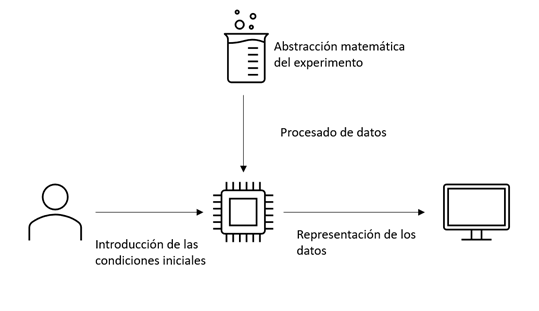
\includegraphics{images/Figura1.1.png}
    \caption{Representación abstracta de simulación.}
    \label{fig:1.1}
\end{figure}

Dada esta motivación, la línea de este trabajo consiste en la elaboración de las simulaciones físicas correspondientes a los \textit{circuitos RC y RL en corriente continua y estado transitorio},  estudiados en la asignatura \textit{Fundamentos Físicos de la Informática} de los grados de \textit{Ingeniería Informática, Software y Computadores} de la \textit{Universidad de Málaga}.

\subsection{Objetivos y metodología}

Como objetivo principal, tal y como se plantea al final del apartado anterior, es ofrecer una solución informática que simplifique el estudio de los alumnos que estudien alguna asignatura de física, en la interpretación de los circuitos RC y RL en corriente continua y estado transitorio. Como toda simulación, tendrá un \textit{engine} (motor) que se encargue de generar los resultados, los cuáles vendrán dados dependiendo de las entradas proporcionadas por el usuario del software, acompañados de animaciones cuya principal función será la de imitar a los circuitos reales. Este será nuestro \textbf{objetivo principal}, así que para alcanzarlo, deberemos de cumplir los siguientes \textbf{objetivos específicos}.\\

Como primera meta, tendremos que realizar un \textbf{análisis matemático} de ambos circuitos, para así obtener un modelo matemático que nos permita expresar analíticamente la evolución de las magnitudes físicas que caracterizan estos sistemas, como la intensidad de corriente de los circuitos, el voltaje de los dispositivos o la energía eléctrica o magnética intercambiada por éstos. Una vez obtenidas estas expresiones, dejaremos a un lado la parte física del proyecto y avanzaremos con la \textbf{evaluación de las soluciones y tecnologías} que nos permitirán desarrollar cada una de las simulaciones y, una vez barajadas todas las posibilidades, el siguiente objetivo será \textbf{aprender la tecnología}. 

Finalmente, nos quedará la \textbf{implementación} haciendo uso de las ecuaciones resultantes del análisis y de la tecnología seleccionada. A este objetivo, le sumaremos una serie de \textbf{pruebas} manuales para comprobar que los resultados obtenidos son los adecuados.\\

Cada uno de estos objetivos planteados, se podría corresponder en cierta manera a cada una de las fases o etapas por la que irá pasando el proyecto hasta finalizarlo. Esta \textit{metodología}, conocida como \textit{incremental} \cite{metodologiasSoftware}, pertenece a los modelos abstractos tradicionales, exactamente a la categoría de los \textit{evolutivos}, entre los que también encontramos otros modelos como \textit{espiral}, \textit{iterativo} o \textit{diseño por planificación}. Todas estas presentan la característica de estar principalmente dividida por cuatro etapas:\\

\begin{itemize}
    \item \textbf{Análisis.} En esta primera fase se llevará a cabo un análisis global del sistema. Es muy importante establecer un diálogo en el que el equipo técnico (desarrollo) y el cliente de la aplicación, pues aquí se tomarán todas las ideas básicas del software, así como la resolución de las dudas que los desarrolladores puedan tener sobre el objetivo esperado del cliente. Además, el planteamiento del proyecto debe de quedar cerrado en esta etapa, salvo en la metodología en espiral (en este caso, el ciclo de desarrollo como su nombre indica es una espiral, por lo que esta etapa sucederá varias veces).
    \item \textbf{Diseño.} \label{software_diseño_etapa} Aquí, es donde se realiza un primer modelo del sistema haciendo uso de los requisitos tomados en la anterior etapa.
    \item \textbf{Implementación.} Como su propio nombre indica, esta etapa consiste en la transcripción a código de las ideas iniciales y obtener como resultado un producto visual de ellas.
    \item \textbf{Pruebas.} Ya completada la implementación, se necesita comprobar que todo funciona correctamente, y para ello se realiza una serie de pruebas generales al software para asegurar que las ideas inicialmente planteadas están perfectamente operativas y no suponen ningún riesgo.
    \item \textbf{Despliegue y mantenimiento}. Una vez el \textit{software} se encuentra terminado y las pruebas realizadas dan como resultado lo que esperábamos, podemos concluir que el producto está listo para su distribución. Sin embargo, al repartirlo entre los usuarios es probable que aparezcan errores que no se tuvieron en cuenta en el momento del diseño y elaboración de las pruebas. Una vez el sistema se encuentre desplegado y sea accesible al público, es necesario llevar un mantenimiento tanto de la aplicación como del \textit{hardware} del servidor dónde se encuentra alojada. Como veremos más adelante utilizaremos un servicio de terceros para realizar el despliegue, así que el mantenimiento \textit{hardware} no depende de nosotros.
\end{itemize}

Normalmente, se suele añadir una quinta etapa llamada mantenimiento. Esta fase final, consiste en una vez desplegado el sistema en una infraestructura, revisar que todo funcione correctamente y, en caso de cualquier imprevisto, encontrar una solución lo antes posible.\\

Para la elaboración de este TFG, se va a emplear una metodología incremental; y aunque no va a tener exactamente la estructura anterior, sí que va a compartir sus fundamentos. Las etapas a llevar a cabo son los siguientes (ver Figura \ref{fig:1.2}):

\begin{enumerate}
    \item Reunión con los tutores.
    \item Investigación de los fenómenos físicos propuestos.
    \item Análisis matemático.
    \item Evaluación de las soluciones y tecnologías.
    \item Aprendizaje de las tecnologías 
    \item Implementación y pruebas.
\end{enumerate}

\begin{figure}[!h]
    \centering
    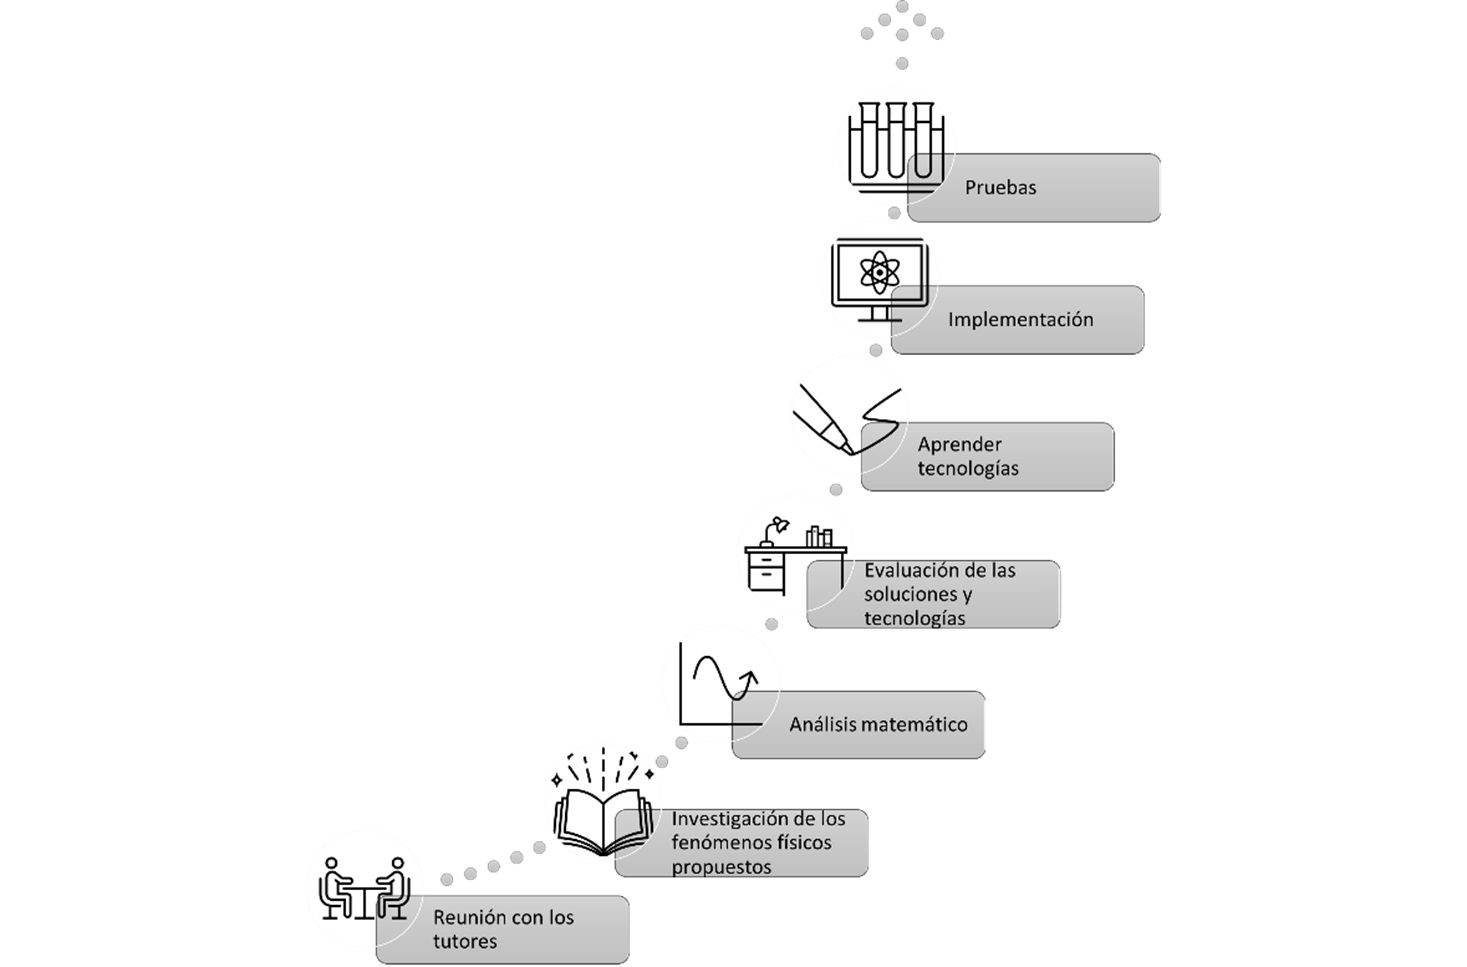
\includegraphics{images/Figura1.2.png}
    \caption{Diagrama de la metodología utilizada. Al estar en una metodología incremental, en cada una de las etapas se van cumpliendo los objetivos propuestos, así como la funcionalidad de la aplicación.}
    \label{fig:1.2}
\end{figure}


\subsection{Estructura del documento}
Por otro lado, siguiendo el orden del desarrollo de las simulaciones, la división de este documento se puede separar en los capitulos mostrados a continuación.

\begin{itemize}
    \item \textbf{Capítulo 1. Introducción. } En esta primera parte, se expondrán las principales motivaciones que llevan a realizar este proyecto, cuáles son sus objetivos finales y específicos, la estructura de la memoria y una breve descripción de cada una de las tecnologías a utilizar durante  el desarrollo.
    \item \textbf{Capítulo 2. Circuitos RC y RL. } En esta segunda sección de la memoria, se realizará un repaso a los fenómenos físicos estudiados, en el que se dará explicación a algunos de sus aspectos clave, los parámetros a estudiar y las ecuaciones que los modelan (todo el desarrollo matemático y físico correspondiente a cada uno de los circuitos se muestra en el apartado de los \textit{Apéndices}).
    \item \textbf{Capítulo 3. Estudio de las tecnologías.} Una vez aclarados los conceptos clave, continuaremos con el estudio de las tecnologías que podrían utilizarse para ejecutar la implementación. Se consideraran varias opciones y será utilizada aquella más conveniente a nuestras necesidades.
    \item \textbf{Capítulo 4. Implementación y pruebas.} Ya seleccionadas y aprendidas las herramientas, seguiremos con la implementación. En este capítulo, se recogerá los principios de estas tecnologías y se aplicarán al caso.
    \item \textbf{Capítulo 5. Conclusión. }Finalmente, se expondrá una conclusión y cómo una breve idea de cómo este trabajo podría extenderse. 
\end{itemize}

\subsection{Tecnologías usadas}
Para terminar con esta primera parte del documento, haremos un repaso de las herramientas que usaremos a lo largo del desarrollo del proyecto. La lista es la siguiente:

\begin{itemize}
    \item \textbf{Visual Studio Code. } \textit{Visual Studio Code} o \textit{VSCode} \cite{vsCode}, es un editor de código desarrollado por \textit{Microsoft}. Una clara diferencia respecto a otros editores, es que éste nos permite la instalación de \textit{plugins} que nos ayudan durante la tarea de programación, como por ejemplo, alerta de errores de sintaxis, la vista del directorio del proyecto actual en forma de árbol (facilidad para ver su estructura) o una terminal incorporada entre otros.
    \item \textbf{Overleaf. }Se trata de una herramienta online, la cuál nos ofrece un entorno de trabajo para elaborar nuestros documentos en \LaTeX, además de un repositorio en el que almacenarlos.
    \item \textbf{Adobe Photoshop. }Es un software para edición de imágenes, cuya principal misión de esta herramienta informática será la elaboración de las animaciones que acompañarán a la simulación.
    \item \textbf{GitHub} es un directorio en la nube que nos permite alojar el código fuente de nuestro proyecto. Además de tener la utilidad de repositorio, nos servirá para realizar el despliegue de la aplicación utilizando el servicio \textbf{GitHub Pages}. 
\end{itemize}

Como vemos, el número de programas informáticos que vamos a utilizar es muy pequeño, puesto que no se necesitan de más. A continuación, se da una lista con los lenguajes de programación y \textit{frameworks} que utilizaremos \footnote{El porqué se utilzan tecnologías orientadas a la programación web, vendrá explicado más detalladamente en el capítulo 3}:

\begin{itemize}
    \item \textbf{HTML. }\textit{HTML} de sus siglas \textit{HyperText Markup Language} \cite{htmldef}, como su propio nombre señala, es un lenguaje basado en etiquetas encargado de definir la estructura básica del contenido de la web. Siempre va acompañado de otras tecnologías como \textbf{CSS} o \textbf{JavaScript}.
    \item \textbf{CSS o \textit{Cascade Style Sheets}. } \cite{cssdef} Se trata de un lenguaje encargado en la presentación de la web. Su finalidad es mejorar la apariencia visual de los bloques escritos en HTML.
    \item \textbf{JavaScript. } Es un sencillo lenguaje de programación \cite{jsdef} utilizado en la mayoría de los sitios Web. Usando solamente HTML y CSS, los documentos generados son estáticos, es decir, su vista es siempre la misma. En cambio, \textit{JavaScript} nos permite dinamizar estas páginas, siendo esto causa de que sea atractiva al usuario. Como veremos más adelante, este lenguaje no se aplica solamente en el \textit{\textbf{front}}\footnote{En una arquitectura web, llamamos \textit{front} o \textit{front-end} al contenido que se ejecuta en el lado del cliente y que por lo tanto, permite interactuar con los servicios que proporciona la aplicación.} de nuestra aplicación, sino también en el \textit{\textbf{back}}\footnote{Llamaremos proceso \textit{back} o \textit{back-end} a aquel que se ejecuta fuera del alcance del usuario de la aplicación, como en un servidor.}.

    \item \textbf{Python. }Se trata de otro lenguaje de programación con una sintaxis bastante similar a \textit{JavaScript}. En este caso, no profundizaremos en detalle en los usos de este lenguaje, pues solamente lo utilizaremos para elaborar un sencillo \textit{script} que se encarga de generar una imagen con los resultados de una simulación sobre un circuito concreto, y así poder compararlos aquellos que obtengamos de la aplicación. Para ello, se hará uso de las librerías de \textit{numpy} \cite{numpy} y \textit{matplotlib} \cite{matplotlib}.
    
\end{itemize}

\begin{figure}[!h]
    \centering
    \subfloat[HTML]{
        \label{f:htmllogo}
        
\includegraphics[width=0.2\textwidth]{images/htmllogo.png}
    }
    \subfloat[CSS]{
        \label{f:csslogo}
        
\includegraphics[width=0.2\textwidth]{images/csslogo.png}
    }
    \subfloat[JavaScript]{
        \label{f:jslogo}
        
\includegraphics[width=0.2\textwidth]{images/jslogo.png}
    }
    \caption{}
    \label{fig:tecnlogos}
\end{figure}

Aunque con las herramientas presentadas hasta el momento se podría construir cualquier vista \textit{front-end}, daremos un paso más y para facilitar la programación del software empleando los siguientes entornos y \textit{frameworks}:

\begin{itemize}
    \item \textbf{NodeJs. }Se trata de un entorno de ejecución \cite{nodejsdef} para \textit{JavaScript} fuera del navegador. Será de utilidad para la instalación de librerías.
    \item \textbf{React.} Es un \textit{framework} \cite{reactjsdef} de programación front-end cuyo principal objetivo es la construcción de la interfaz de usuario mediante la reutilización de componentes. Utiliza NodeJs como entorno de ejecución y JavaScript como lenguaje principal.
    \item \textbf{Bootstrap. }Durante el desarrollo de la aplicación, veremos que CSS puede complicarse bastante cuando queramos posicionar elementos en un lugar concreto de nuestra pantalla. Bootstrap \cite{bootstrapdef} se encargará de facilitarnos esto, además de la creación de componentes básicos (botones, enlaces, \textit{grid-layout}, ...) con estilos predefinidos. 
\end{itemize}


\end{document}